\documentclass[a4paper,12pt]{article}

\usepackage{url}
\usepackage{epsfig}
\usepackage{graphics}
\usepackage{fancyhdr}
\usepackage{listings}
\usepackage{booktabs}
\usepackage{lastpage}


\graphicspath{{pictures/}}

\title{Word prediction performance of n-gram models applied to  different corpora}
\author{\hspace*{-0.5cm}
GROUP 34\\
\begin{tabular}{cccc}
Sofia Broom\'e & Jeremy Krebs & Valentin Geffrier & Erik Fredriksen \\
901210 & 920421 & 921104 & 860328 \\
sbroome@kth.se & jeremyk@kth.se & geffrier@kth.se & efred@kth.se \\
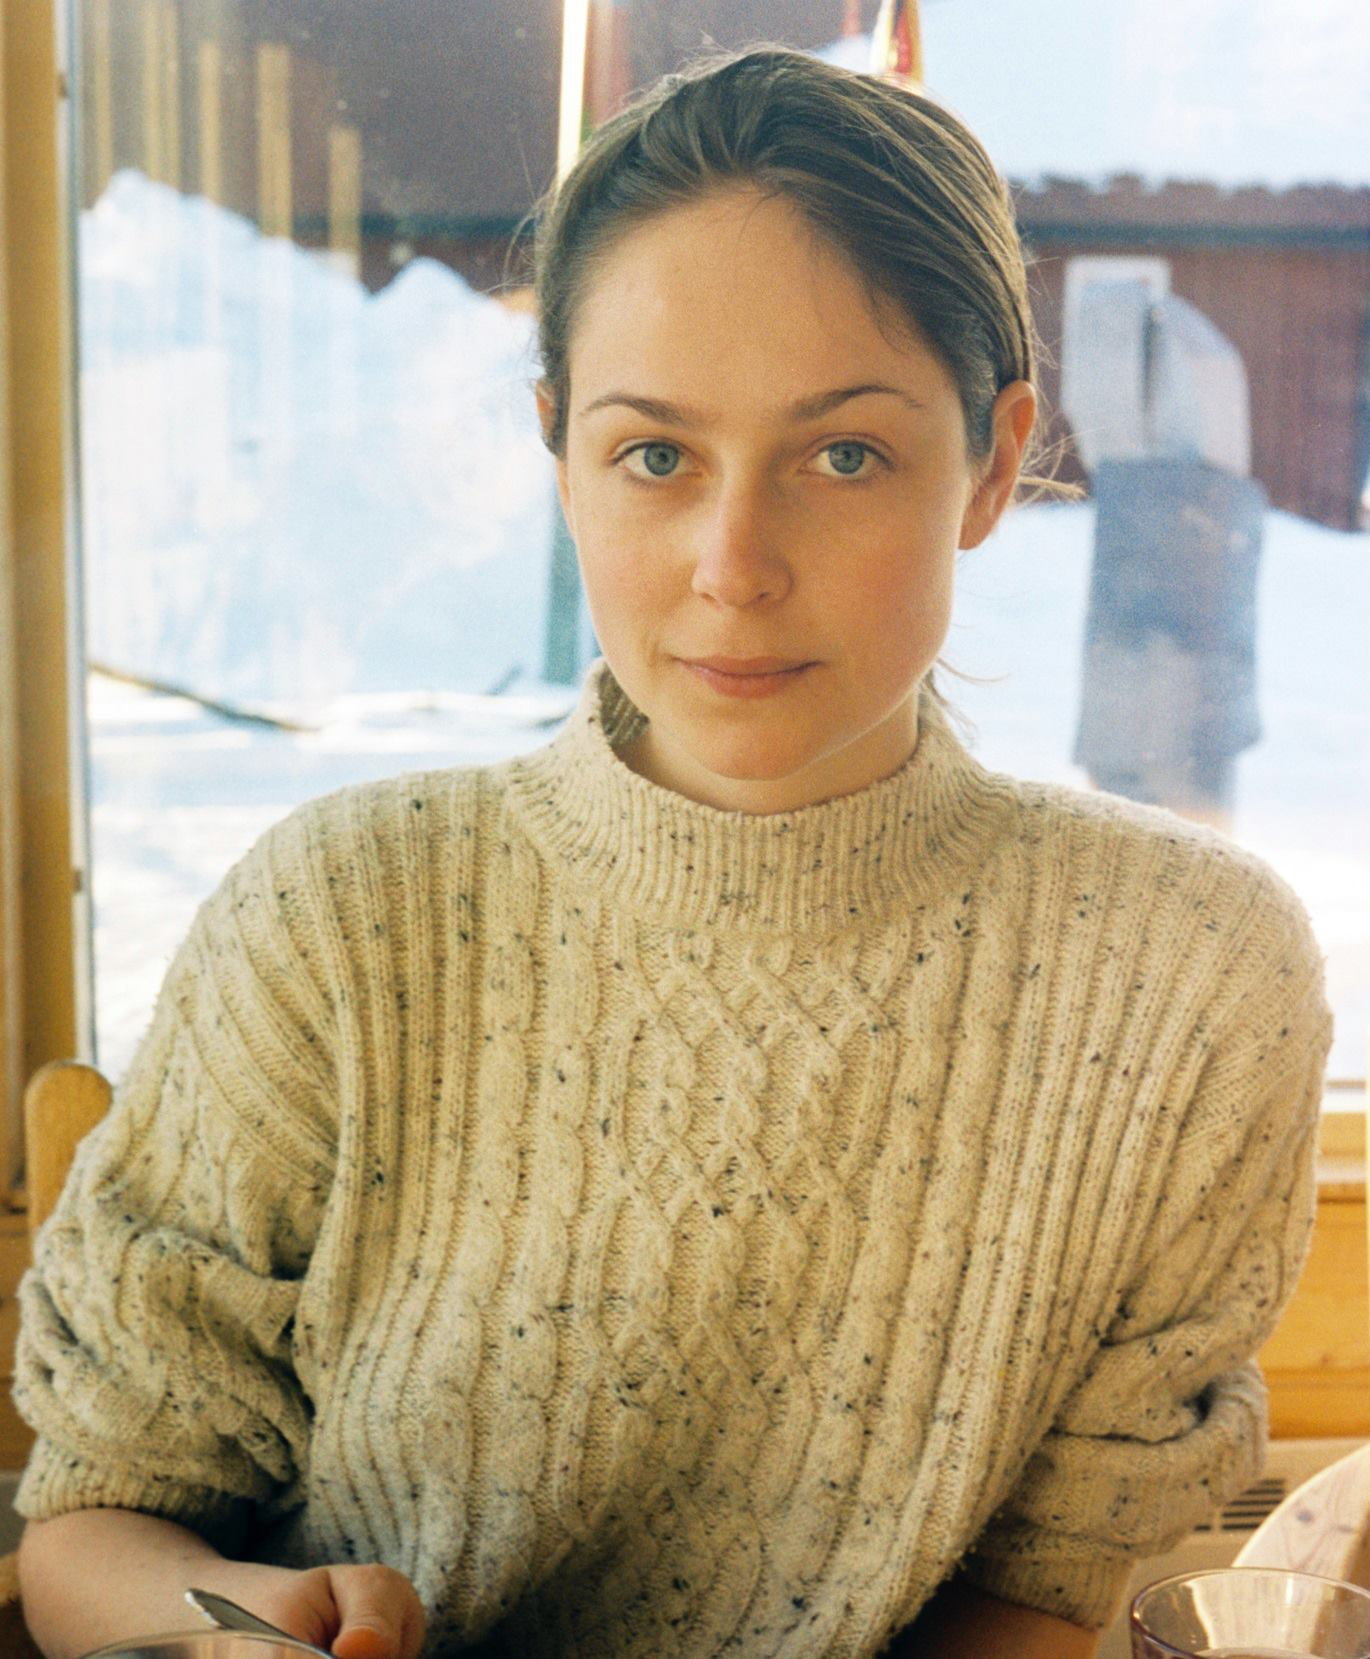
\includegraphics[width=0.16\linewidth]{Nikkaluokta} & 

\includegraphics[width=0.19\linewidth]{jrm} & 
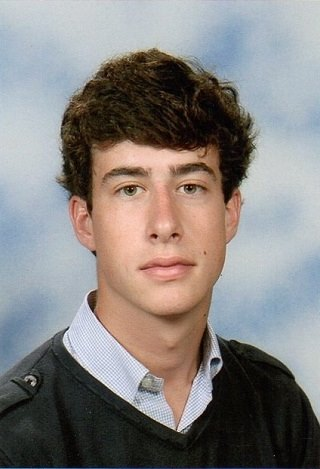
\includegraphics[width=0.13\linewidth]{geff} & 
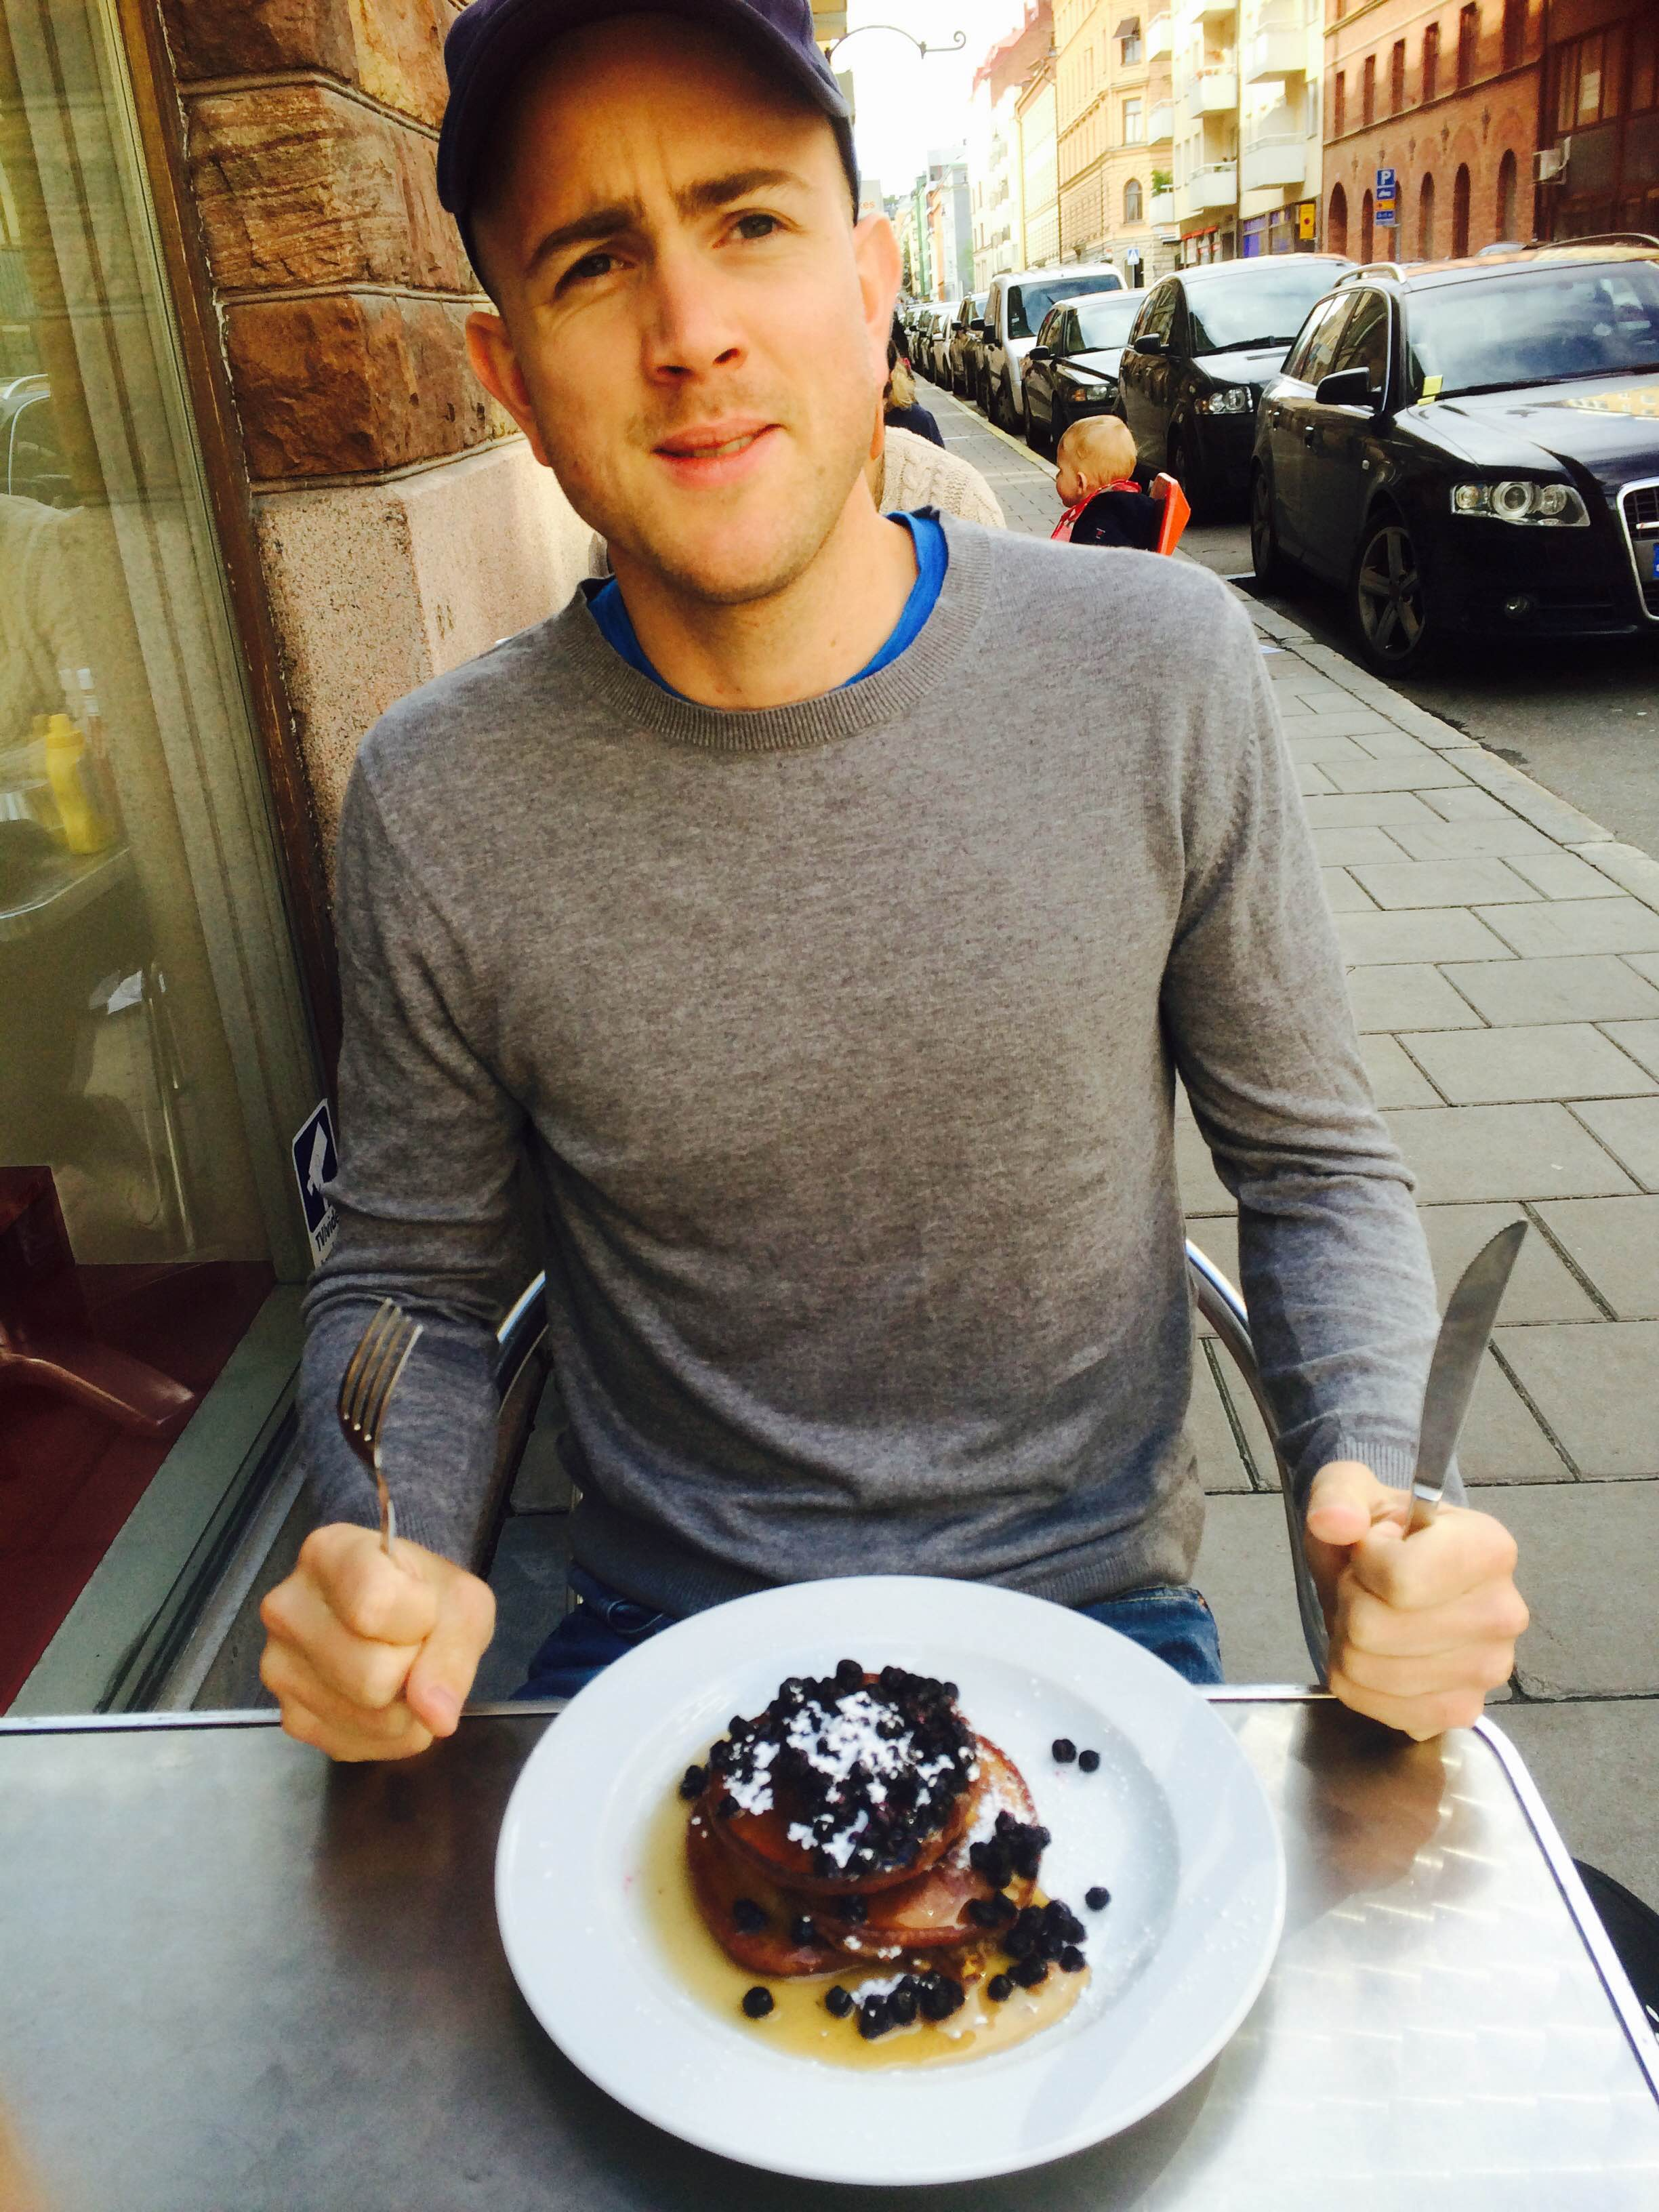
\includegraphics[width=0.15\linewidth]{erikpancakes}
\end{tabular}} 

\date{}

\pagestyle{fancy}
\setlength{\headheight}{15pt}
\fancyhf{}
\cfoot{\thepage / \pageref{LastPage}}
\lhead{DD2380 ai15} % DO NOT REMOVE!!!!
\rhead{S. Broom\'e, J. Krebs, V. Geffrier, E. Fredriksen} %% UPDATE WITH YOUR NAMES

\begin{document}

\maketitle
\thispagestyle{fancy}

\begin{abstract}
The goal of this project was to predict words to continue a word sequence. Going from simple bigram models to more complex n-gram models using different smoothing methods and grammar constraints, we have been able to improve the performances of our predictor on different types of corpora. N-gram models need additional layers consisting of smoothing techniques and grammar constraints to be more credible as word predictors. The performance of our system relies not only on the length of our n-gram model but also on its customization with smoothing, grammar constraints, the size of the training corpora and its similarity to our input.
\end{abstract}



\clearpage

%%%%%%%%%%%%%%%%%%%%%%%%%%%%%%%%%%%%%%%%%%%%%%%%%%%%%%%%%%%%%
%%%%%%%%%%%%%%%%%%%%%%%%%%%%%%%%%%%%%%%%%%%%%%%%%%%%%%%%%%%%%

\section{Introduction}
\label{sec:intro}
Being able to dissect, classify, analyze and reproduce language is a highly relevant task for various fields. In the realm of artificial intelligence, we want to give language to our agents by means of communicating with them. When we deal with natural language processing we say that we make language models. Seen as there is no finite set of rules that can describe, say, the entire English language in a complete sense, the prevailing method is to approximate language by probabilistic methods.

N-grams are the building block for almost every language model. An n-gram is simply a tuple of n co-occuring words, and the probability distribution of these tuples (according to some collection of words) constitute our model of the language. This  simple construct captures many patterns in language. Grammar is not taken into account explicitly, but local context will inevitably be built in. For instance, an adjective will in many cases be followed by a noun, or a pronoun by a verb, and thus a bigram composed of those two grammatical types in the mentioned order will score high in probability.  Gao and Suzuki\cite{gao2004long} explore long distance dependency for words through word clusters and the linguistically motivated {\it function word skipping} method where function words such as "has", "a", "in", "and", "the", etc, are skipped in favor of more significant words, called head words

There are some practical issues with the n-gram model. Perfectly valid n-grams missing from the training corpus will be given a zero probability. Smoothing techniques are an attempt to tackle this issue. Higher-order n-gram are particularly prone to sparseness, so we might want to "back off" from the n'th order and approximate it with a weighted sum of lower order n-grams. 

Furthermore, what kinds of test sets does our training set allow us to perform well on? One should train on a  corpus which is representative of the domain of the intended use. And what happens to our model when we apply it to languages with a higher degree of inflection? We train on English text, but languages like Swedish, Basque or German have been shown to perform worse \cite{garay2006text} .

From the above examples we see that in many cases just using the n-gram model in itself will not suffice. Over the years, researchers in natural language processing have added a lot of tweaks to the original idea; cache language models, LSA-based language models and maximum entropy models, to name a few.

In what follows we will explore n-gram models of varying degrees on corpora and grammar to see which results are obtained under which circumstances.

\subsection{Related works}
We began our exploring of natural language processing through the Natural Language Toolkit website and the accompanying book, Natural Language Processing with Python. The theory to accompany the more practical methods from NLTK was mainly obtained from Daniel Jurafsky and James H. Martin's 1999 book Speech and Language processing \cite{JurafskyBook}. Daniel Jurafsky also has made a series of video lectures on the subject for a Coursera online course. From \cite{brown1992class} and \cite{garay2006text} we got a sense of the challenges of extending the concept of n-grams, as well as for modern applications of text prediction.

\subsection{Outline}
The lion's share of the report consists of three sections, hereunder, concerning respectively n-gram models, n-gram models with smoothing and n-gram models with grammar constraints, where each of them contains some theory, accounts of our related experiments and results and discussions of possible issues. In the end there is a summary and conclusion.

%%%%%%%%%%%%%%%%%%%%%%%%%%%%%%%%%%%%%%%%%%%%%%%%%%%%%%%%%%%%%
%%%%%%%%%%%%%%%%%%%%%%%%%%%%%%%%%%%%%%%%%%%%%%%%%%%%%%%%%%%%%
%%%%%%%%%%%%%%%%%%   NGRAM MODELS   %%%%%%%%%%%%%%%%%%%%%%%%%
%%%%%%%%%%%%%%%%%%%%%%%%%%%%%%%%%%%%%%%%%%%%%%%%%%%%%%%%%%%%%
%%%%%%%%%%%%%%%%%%%%%%%%%%%%%%%%%%%%%%%%%%%%%%%%%%%%%%%%%%%%%
\section{N-gram models}
\label{sec:ngram}

\subsection{Theory}
The first mathematical tool needed in all natural language processing experiment is n-gram models. Speech taggers, smoothing and other methods may not be implemented at first, but n-gram models are needed to predict the next likely words of a sentence.

These models are quite easy to understand: if n is a fixed integer, a n-gram model works as a Markov chain to predict the next word. A model is trained on a corpora C, for instance a book or a set of books, so that the probability of each n-gram in the language is learned by the model. The bigger the corpora the more accurate and reliable will be the model as it will have more data to compute probabilities of sequences. More precisely, the probability $p$ that the word $w_n$ follows the group of words $w_1 w_2 ... w_{n-1}$ is given by the following formula:

$$ p = p(w_n | w_1 .. w_{n-1}) = \frac{|{(w_1, .., w_{n-1}, w_n) \in C}|}{|{(w_1, .., w_{n-1}, x) \in C}|} . $$

This makes it possible to predict a likely next word, but also to generate the end of the sentence, each new word selected using the probability distribution. Therefore, an n-gram which appeared a lot in a corpora is more likely to appear in the sentence generator. However, this also tells us that heuristically, we should expect different results from one corpora to another. The length of the corpora is to take into consideration since the idea is to train the model. The corpora we used have between 10,000 and 1,000,000 words. Another point is that using corpora from Shakespeare, the generated sentences are likely to be more erratic than with a novel since Shakespeare's syntax and grammar are more complicated. For modernist poetry like Whitman's Leaves of Grass it turns out to work quite well with a basic n-gram model, since the somewhat abstract resulting sentences fit with the textual situation and since the verse structure isn't as demanding as in shakespearian texts. Poetry has higher context satisfaction for a crude n-gram model.


\subsection{Experimental results}
\subsubsection{Parameter $n$}
	The first experiment we did was to try to understand the influence of n in our word predictor and how we could tune this parameter. In these experiments, only the corpora and n is changed - no parts-of-speech-tagger or smoothing have been used. The table \ref{tab:corpus2} shows n-gram predictions of the end of the sentence "Alice was looking for" for $ n\in(2,4) $.
	
We should note that a 1-gram model is not a Markov model. It just predicts a word according to its frequency in a book. As punctuation symbols are considered as words in this corpora, that explains why it predicts so many commas and apostrophes. 

A 2-gram model will only predict a word according to the immediately preceding word in the sequence. This explains why after words like "the" and "a" there are often adjectives or nouns. However, the prediction is still not perfect because of the short reach of the model.

With 3-and-4-gram models one can see that the sentences are a bit more grammatically correct but there is still some issues since the English grammar and syntax are not used in these models. Another thing with 4-gram models is that we can see the predictions are quite close to each other for different attempts. This is because the more words are fixed, the less freedom there is for the next word: there are fewer bigrams starting with "for" than 4-grams starting with "was looking for" in the corpora.

If n is too low, the predictor will be inferior because one or two words might not be enough to predict a likely next word. However if n is too big, the corpora needs to be really extensive as well and contain enough different n-grams so that the predictor is more diversified.

\subsubsection{Example}

\begin{table}[!h]
\small
%\begin{center}
\begin{tabular}{| l |c|}
\hline
Query followed by 10 generated words & $n$ \\ \hline
"Alice was looking for a very neatly spread his belt and began . ' " & 2\\ \hline
"Alice was looking for I wish I don ' And with a lobster as" & 2\\ \hline
"Alice was looking for I ' Well , but I ' m a dance" & 2\\ \hline
"Alice was looking for eggs , I can kick a little bottle that stood "& 3 \\ \hline
"Alice was looking for the White Rabbit blew three blasts on the look of"& 3 \\ \hline
"Alice was looking for the garden , among the bright eager eyes were nearly"& 3 \\ \hline
"Alice was looking for the fan and gloves . ' How queer it seems" & 4 \\ \hline
"Alice was looking for the fan and a pair of white kid gloves , " & 4 \\ \hline
"Alice was looking for the fan and gloves , and she very good -" & 4 \\ \hline
\end{tabular}
\caption{Corpus 2}
\label{tab:corpus2}
%\end{center}
\end{table}


%%%%%%%%%%%%%%%%%%%%%%%%%%%%%%%%%%%%%%%%%%%%%%%%%%%%%%%%%%%%%
%%%%%%%%%%%%%%%%%%%%%%%%%%%%%%%%%%%%%%%%%%%%%%%%%%%%%%%%%%%%%
%%%%%%%%%%%%%%%   SMOOTHING   %%%%%%%%%%%%%%%%%%%%%%%%%%%%%%%
%%%%%%%%%%%%%%%%%%%%%%%%%%%%%%%%%%%%%%%%%%%%%%%%%%%%%%%%%%%%%
%%%%%%%%%%%%%%%%%%%%%%%%%%%%%%%%%%%%%%%%%%%%%%%%%%%%%%%%%%%%%
\section{N-gram models with smoothing}
\subsubsection{Initial practical problems: an SRILM excursion}
Building a full-fledged language model in Python is not a trivial endeavor (this could be a project in itself). We thought NLTK provided the facilities to accomplish this, but it turned out this module had been deprecated due to bugs. 

The online toolkit SRILM provided by the Stanford Research Institute is an extensive framework, also evidently widely adopted - the introductory SRILM article by Andreas Stolcke has over 3 000 Google Scholar citations.

SRILM itself is a library of C++ classes, but contains ready-made command line tools. For example, invoking "ngram-count" on the Moby Dick corpus from NLTK (where corpus.txt has been parsed to match SRILMs format: one sentence per line with tokens separated by whitespace) produces an ngram language model of this text, with Good-Turing discounting and Katz backoff for smoothing.

Doing actual predictions with this framework proved to be a bit harder, we found a Python wrapper (pysrilm) that was supposed to provide this functionality, however, it was a Cython extension that needed to be compiled and linked against the SRILIM library. This did not work, so we returned to our own Python n-gram model to implement a smoothing method ourselves.

\label{sec:ngramsmoothing}

\subsection{Theory}
	The issue behind simple n-gram models is that the maximum likelihood estimate only consider n-grams in the corpora. That is, many n-grams are not considered by the model to have a strictly positive probability because there is sparsity in the data. However in most cases one does not want to give a zero probability to an unseen event since an event that did not occur in the training data could occur in the test data. Smoothing methods are used to adapt the probability distribution so that unseen events have a probability greater than 0. There are different ways of smoothing and we experimented with mainly three methods implemented in $nltk$:
	
	\begin{description}
		\item[Witten-Bell:] This method gives the same probability mass to the unseen events as the total probability mass of the events seen exactly once in the corpora. There are usually a lot more unseen events than events that occured once, thus the model seems reliable because it will give a low probability to the unseen ones. A given parameter is the number of total events, seen or unseen. If there are $m$ unique words in the corpora and we are considering n-grams, the parameter will not necessarily be as big as $m^n$ since the corpora could be lacking words that we want to add manually, or we can ignore some n-grams because they are not valid grammatically.
		\item[Lidstone:] This method simply adds a value $\gamma$ to the frequency of all events. It then computes the basic maximum-likelihood probability based on those new frequencies. This parameter, is commonly set to around 0.5 but can be tuned. With that value, the weight of an unseen event will be a third of the weight of an event that occured once. We can note that this method derives from the Laplace smoothing method which is when $\gamma = 1$.
		\item[Good-Turing:] A more complicated method that gives the same probability to the events that occured $n$ times as to the events that occured $n+1$ times. With high values of $n$ it can happen that no event occured that many times. For these events, an estimation is done. In NLTK, the number of events that occured $n$ times is estimated to be $N(n) = an^b$ where $a$ and $b$ are estimated using linear regression on the logarithm of the equation: $log\ N(n) = log\ a + b\ log\ n$.
	\end{description}
	
	\subsection{Experimental results}
	
	In the following experiments, we tried to point out how smoothing methods could change the probability distribution of the n-grams for our predictor. We also compared the sentences with or without smoothing, but looking at the actual numerical probabilities makes more sense to understand how smoothing methods work. Three n-grams of different frequencies in the corpora served as illustrative examples for how their (respective) probabilities were changed with smoothing.
	
\subsubsection{The probability distribution}
	In figure \ref{fig:smoothingdist}, we tried to see what impact the three above techniques had on the probability distribution of the 2-grams and 4-grams for the corpora "Alice in Wonderland". The n-grams with low frequency are not considered here as their probability is roughly the same after smoothing. As we could expect, the blue (smoothed) graphs are generally lower than the red (unsmoothed) because probability weight is taken from seen events to unseen events. The mass distribution however varies between the different methods; the Lidstone probability for instance does not take the same weight from all n-grams. With our parameters, Good Turing doesn't change much of the probability distribution from the unsmoothed case, from which we conclude that the tuning of the parameters is important. We should also take the size of the corpora into account as the ratio between the number of unseen events and seen events has a crucial effect in the computation of probabilites.

\begin{figure}
	\label{fig:smoothingdist}
	\begin{tabular}{cc}
		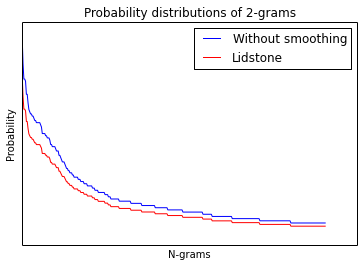
\includegraphics[width=0.52\linewidth]{2_Lidstone} & 
		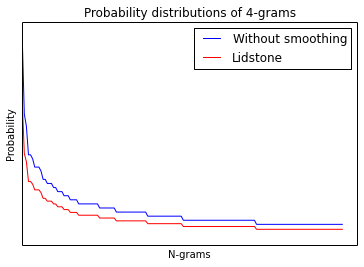
\includegraphics[width=0.52\linewidth]{4_Lidstone} \\
		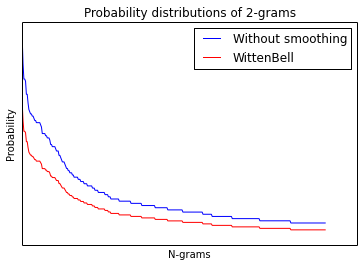
\includegraphics[width=0.52\linewidth]{2_WittenBell} & 
		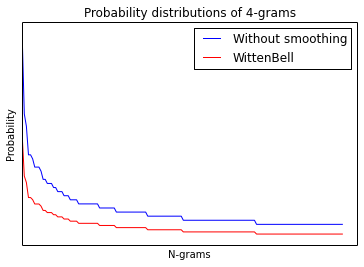
\includegraphics[width=0.52\linewidth]{4_WittenBell} \\
		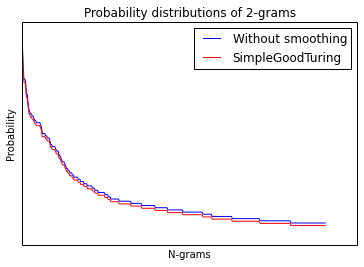
\includegraphics[width=0.52\linewidth]{2_Turing} & 
		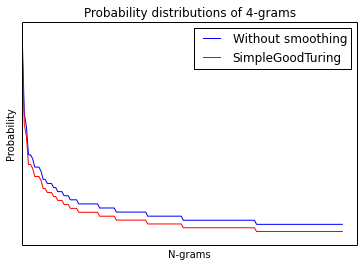
\includegraphics[width=0.52\linewidth]{4_Turing} \\
	\end{tabular}
	\caption{Changes of the probability distribution for different smoothing methods}
\end{figure}

\subsubsection{Specific example}
	Table \ref{tab:smoothingprobs} shows the probability and probability ratio change of three bigrams from the same corpora: (she, was) with a frequency of 49, (she, is) of count 3 and the unseen (she, blue). Zero probabilities as removed as intended. We can however see the ratio of the probabilities between (she, was) and (she, is) change differently depending on the method. If Witten-Bell does not change it, Lidstone and Turing does as they do not allocate the same weight percentage of each seen event to the unseen ones.

\begin{table}[!h]
\small
\centering
\caption{Data for different smoothing techniques}
\label{tab:smoothingprobs}
\begin{tabular}{@{}lllll@{}}
\toprule
Smoothing:     & None      & SGT       & WB        & LSPB 0.5   \\ \midrule
P(she, is)     & 8.795e-05 & 6.072e-05 & 6.025e-05 & 8.343e-05  \\
P(she, was)    & 0.001437  & 0.001396  & 0.0009841 & 0.001180   \\
P(she, blue)   & 0.000     & 3.701e-08 & 3.469e-08 & 1.192e-05  \\
Ratio was/is   & 16.33     & 22.99     & 16.33     & 14.14      \\
Ratio was/blue &           & 37710     & 28370     & 99.00      \\ \bottomrule
\end{tabular}
\end{table}

\subsection{Issues}
	The last example can show how careful one needs to be when it comes to smoothing. If the parameter is badly tuned, the probability of an unseen event such as (she, blue) can be high regardless of its obvious grammatical problems. We can thus conclude that n-gram models simply in combination with smoothing technics cannot grasp the complex syntax, grammar and structure of language: we need grammar constraints if we want to improve.


\section{N-gram models with grammar constraints}
\label{sec:ngramgrammar}

\subsection{Theory}

The standard approach to grammar in language modeling is to tag every word in a corpus with so called parts-of-speech-tags, sorting the tokens into categories like noun, verb, adjective, determiner, pronoun, adverb, conjunction, etc. Even punctuation is a category among the parts-of-speech, since it is a particular token that has predictive power. Punctuation encodes grammatical structure. The tagging can be challenging since one word can have varying grammatical roles and semantic meaning depending on its syntactic location. Different tagsets can be used depending on how fine grained you want your model to be, but broadly speaking they can be divided into two categories: rule-based taggers and stochastic taggers. Rule-based taggers are decided according to a set of explicitly written rules that were made to dodge tagging ambiguities. Stochastic taggers on the other hand can function like decision trees orientating through probabilistic features or Hidden markov models where for instance an applied Viterbi algorithm can choose the word-and-tag-path with the highest likelihood. The use of HMMs when working with POS-tagging started in the 1980s. 

\subsection{Experiments}

So far our n-gram model word predictor have often given us an answer that doesn't fit in syntactically. Because of this we decided to make of use the nature of each word to perfect our predictions. We tried a simple approach: by creating a new "text" from all the parts-of-speech-tags (POS-tags) associated to the original words of the text we could train a "meta" m-gram model on just the long sequence of tags. Then, we trained an n-gram model on the text. For the "tag text", m can be higher than when we work with normal corpora since a lot of completely different word sequences can be hidden behind the same POS-tag sequence.

For the tag-prediction, we can build an m-gram model where $m \ge n$ that gives the probability of having a particular POS-tag after the sequence of tags corresponding to our word sequence. In our grammar model, we decided to multiply the probability of an n-gram word sequence with the probability of the m-gram tag sequence where the last tag corresponds to the last word. This method changes the original results and makes some sequences more probable than others, given this new grammatical information.

\begin{table}[]
\centering
\small
\caption{Words generated with grammar constraints}
\label{grammarsent}
\begin{tabular}{| l |c|}
\hline
Query followed by 10 generated words                                   & n \\ \hline
Alice was looking for some curiosity . Then the Rabbit . CHAPTER IX .  & 2 \\ \hline
Alice was looking for the voice behind a sulky tone , twinkle --"' and & 2 \\ \hline
Alice was looking for a bat , that : and take the earth .              & 2 \\ \hline
Alice was looking for some time to be in a sort of the book            & 2 \\ \hline
Alice was looking for eggs , as well go in at the Duchess ;            & 3 \\ \hline
Alice was looking for eggs , as the whole court was a dispute going    & 3 \\ \hline
Alice was looking for eggs , as the game . The judge , would           & 3 \\ \hline
Alice was looking for the Duchess began in a day at school , too       & 3 \\ \hline
Alice was looking for the garden : the others looked round also , and  & 3 \\ \hline
Alice was looking for the fan and gloves , and , as the game           & 4 \\ \hline
Alice was looking for the fan and a pair of gloves and a fan           & 4 \\ \hline
Alice was looking for the fan and a pair of the gloves , and           & 4 \\ \hline
Alice was looking for the fan and the pair of white kid gloves in      & 4 \\ \hline
Alice was looking for the fan and the pair of white kid gloves while   & 4 \\ \hline
Alice was looking for the fan and the pair of white kid gloves ,       & 4 \\ \hline
\end{tabular}
\end{table}

\subsection{Issues}

Without smoothing, the same problem as before remains: zero probabilities for unseen events (be it tags or words). To resolve this, we can use the same smoothing that we used previously and have better results. Our method does not rely on a mathematical explanation but it still allows us to take into consideration the grammar, at a deeper level than for words, at the only condition that we use corpora which have the same grammar type as the text we want to complete, to train our n-gram model on. Indeed, we know that the syntax can be completely different in poetry, Shakespeare works or novels. It was already true when we did not use grammar but it becomes absolutely necessary here or the grammar prediction would just make the performance of our results decrease.
Using parse trees could be an improvement to model grammatical sentence structure, as it is more precise to use a more detailed context than only POS tags.

%%%%%%%%%%%%%%%%%%%%%%%%%%%%%%%%%%%%%%%%%%%%%%%%%%%%%%%%%%%%%
%%%%%%%%%%%%%%%%%%%%%%%%%%%%%%%%%%%%%%%%%%%%%%%%%%%%%%%%%%%%%
\section{Summary and conclusions}
\label{sec:summary}

In order to predict the next and following word of a sentence, we trained n-gram models on several corpora of English text.  We extended our model by incorporating part-of-speech tags to produce grammatically correct sentences, and smoothing to handle unseen words. 
We find that the training corpus (more similar to the prediction genre is better), smoothing, and grammar constraint all contribute to the effectiveness of our model.  Further extensions could focus on the implementation (efficient data structures to handle large models), or large grammars to validate syntactically correct sentences.

\nocite{*}
\bibliographystyle{plain}
\bibliography{reflist}



\end{document}
